%
% Modified by Sameer Vijay
% Last Change: Wed Jul 27 2005 13:00 CEST
%
%%%%%%%%%%%%%%%%%%%%%%%%%%%%%%%%%%%%%%%%%%%%%%%%%%%%%%%%%%%%%%%%%%%%%%%%
%
% Sample Notre Dame Thesis/Dissertation
% Using Donald Peterson's ndthesis classfile
%
% Written by Jeff Squyres and Don Peterson
%
% Provided by the Information Technology Committee of
%   the Graduate Student Union
%   http://www.gsu.nd.edu/
%
% Nothing in this document is serious except the format.  :-)
%
% If you have any suggestions, comments, questions, please send e-mail
% to: ndthesis@gsu.nd.edu
%
%%%%%%%%%%%%%%%%%%%%%%%%%%%%%%%%%%%%%%%%%%%%%%%%%%%%%%%%%%%%%%%%%%%%%%%%

%
% Chapter 4
%

\chapter{DATA ANALYSIS}
\label{chap:dataAnalysis}
We care about two things:
1. The absolute cross-section of the ground state transition
2. Setting a limit on excited 0+ state cross-sections

error calculations: its own section?

\section{Detector Efficiency}

deuterium, Mg, cuts

\section{Experimental Parameters Related to the Cross Section}
current, tgt thickness (RBS), solid angle, dead time
go ahead and discuss errors while you discuss these quantities

The absolute cross section is the number of times a reaction occurred normalized by the total number of particles incident on the target and the number density of nuclei in the target:

\begin{equation}
\text{cross section} = \frac{\text{times reaction occurred}}{\text{particles incident on target} \times \text{number density of target nuclei}}
\text{cross section} = \frac{\text{times reaction occurred}}{\text{particle current} \times \text{time} \times \text{target thickness}}
\label{eq:cross_section}
\end{equation}

\section{Background Subtraction}

two data sets
- pulse selection
- no pulse selection

background
- gamma peaks - do not overlap with neutron peak
- other neutron peaks - ??
- randoms - background in both data sets
- continuum - more important in non-pulse-selected data

extracting counts 
- pulse selection
- no pulse selection

The data sets for this analysis were gathered in two seperate runs; the pulse selector was not working for part of the first run.  Analysis of the datasets taken with pulse selection is straigtforward and will be discussed first.  Without pulse selection, the neutron peak sits on top of background from previous neutron bunches.  The background fit is different and the total counts have a larger systematic uncertainty; extracting these will be discussed second.

\subsection{Pulse-Selected Data}
Consider the signals that build the TOF spectrum.  Random background radiation can occur at any time with respect to the beam bunch.  In fact, it should have no knowledge of the beam bunch and is equally likely to occur at every time after a beam bunch.  In other words, the TOF spectrum of background radiation should be flat.  Taking a TOF spectrum with no beam confirms this.

%figure of beam-off TOF spectrum

The neutrons coming from the ground state of \As{78} are monoenergetic and should come at a fixed time relative to the beam bunch; counts from these neutrons should form a peak that is approximately as narrow in time as the beam bunch.  Looking a a beam-on TOF spectrum, it is clear that the neutron peak and the flat background are not the only features.

% figure of beam-on TOF spectrum

The other prominant features of this spectrum are peaks from gammas produced when the beam hits the target and also neutrons from excited states as well as a broad neutron evaporation spectrum from multiple-channel interactions.

In the case of the pulse-selected data, the background that overlaps with the neutron peak of interest is well-determined.  The gamma peaks are far away from the neutron peak and have no effect.  Wonderfully, the broad, flat region ennables a very precise estimate of the random background level.  The neutron evaporation peak is the least-well understood contributor to the background of the ground state neutron peak and will be discussed later.  For now, we focus on the simplest contribution to the background, the flat distribution due to randoms.

In general, extracting the counts due to the neutrons is simple:

\begin{equation}
\text{Sum(peak region) - Background(peak region)}
\label{eq:counts}
\end{equation}

With an associated error

\begin{equation}
\sqrt{\sigma_{Sum}^2 + \sigma_{background}^2}
\label{eq:errDef}
\end{equation}

The sum of counts in a fixed region can be understood as a random variable; as such, its error is $sqrt(N_{peakregion})$.  This is quite large - is there an extraction method that will reduce this error?  The two most straightforward options available to a physicist bent on extracting counts due to a signal are sideband subtraction and fitting.  Fitting when the background is not understood can lead to systematic errors, while sideband subtraction's accuracy depends on a background that does not change rapidly near the signal region.  With these data sets, the number of signal counts is very small compared to the background.  Using sideband subtraction introduces another random variable and increases the width of the distribution of extracted counts for a given bar.  In the case of the pulse-selected data, there is no need to introduce this additional statistical error because the flat background is determined to within ??\%, so that using the fitted value is much more like introducing a constant into the equation for the extracted counts, improving the fractional error by almost a factor of $\sqrt{2}$.  See \fig \ref{fig:statDist} to see the effect of using the fitted value on the width of the extracted count distribution.

\begin{equation}
Counts = Sum(peak region) - Fitted Constant * number of Bins
\sigma^2 = Sum + fit error
\label{eq:fitErr}
\end{equation}

\begin{figure}[ht]
\centering
  \subfloat[Distribution of Background Counts][Distribution of Background Counts]{
  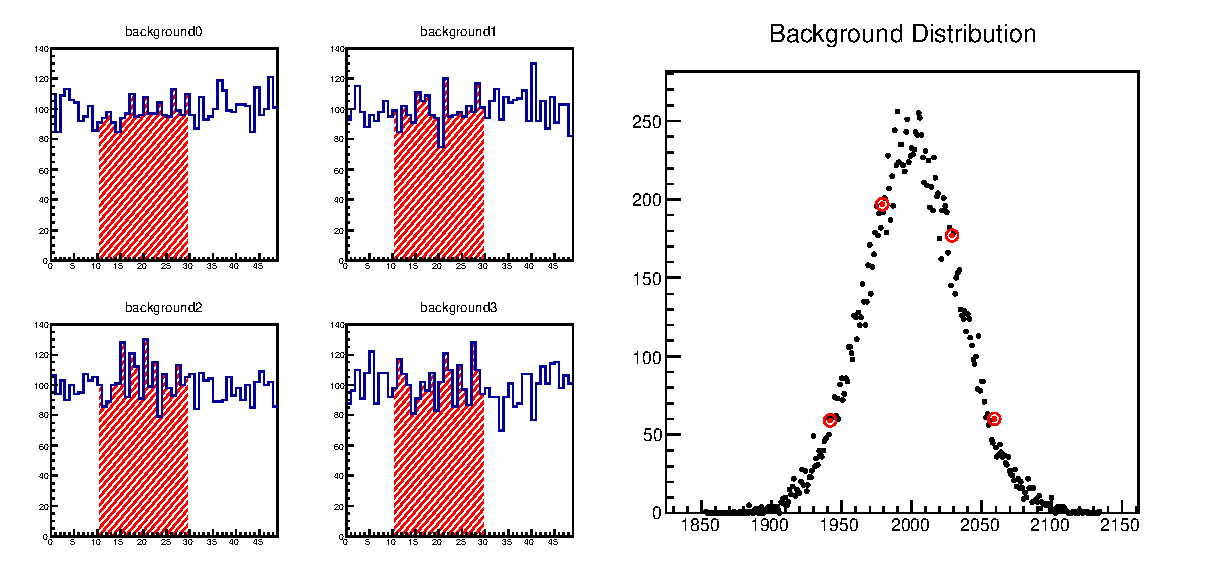
\includegraphics[width=0.3\textheight]{figures/bkgDist}
  \label{fig:bkgDist}}
  
  \subfloat[Distribution of Signal Counts][Distribution of Signal Counts]{
  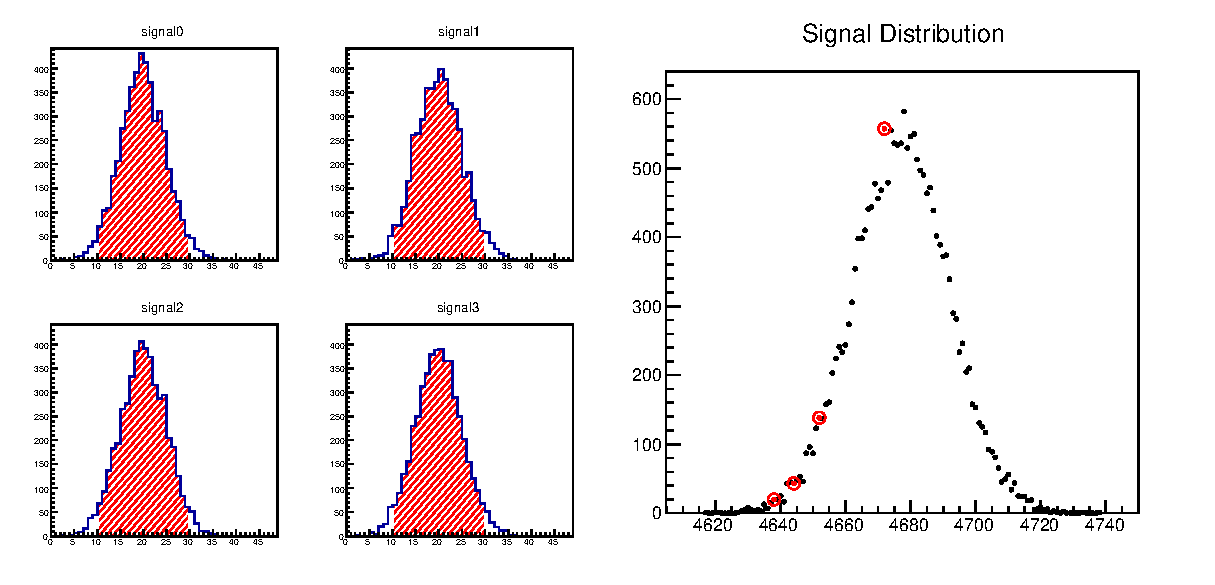
\includegraphics[width=0.3\textheight]{figures/sigDist}
  \label{fig:sigDist}}
  
  \subfloat[Distribution of Extracted Counts][Distribution of Extracted Counts]{
  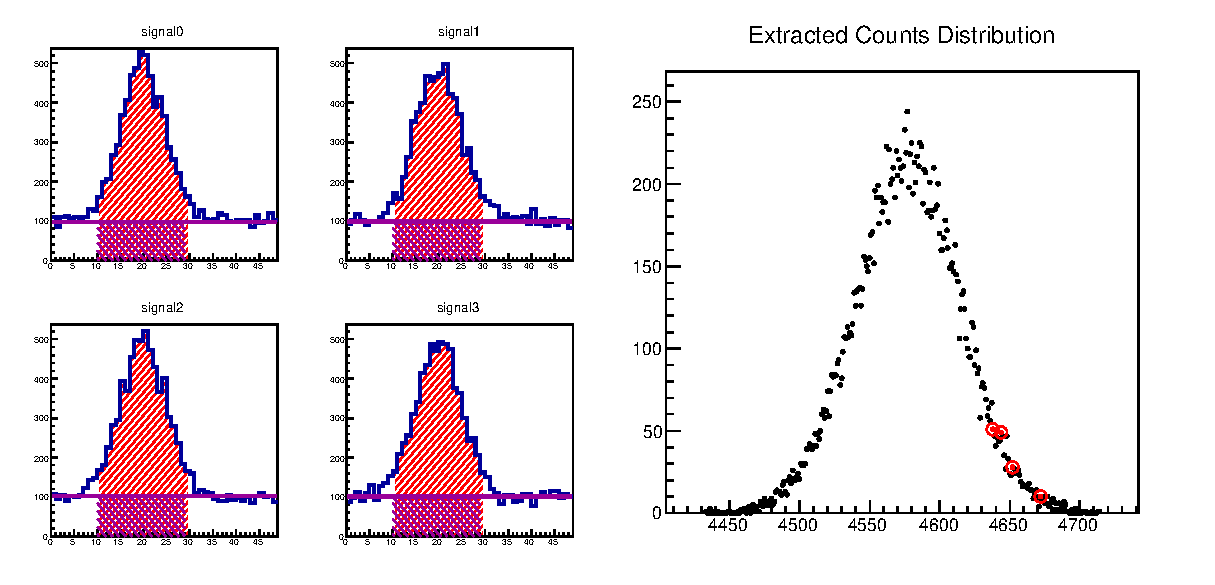
\includegraphics[width=0.3\textheight]{figures/extractDist}
  \label{fig:extractDist}}

  \caption{The number of counts in the peak region are a sum of the number of counts in the random background and counts from the neutrons.  The width of a sample at a uniform rate is simply sqrt(N), as seen in figure ??.  This is an appropriate description of the random background.  The neutron peak is roughly gaussian-shaped, and running trials where counts are drawn from a gaussian distribution shows that the width is ??.}
  \label{fig:statDist}
\end{figure}

The error introduced to the extracted counts depends on how the background is determined.  In the case of the pulse-selected data, it is clearly better to fit the background.  The constant component of the background is well-determined and contributes a tiny ??\% to the total error.  The evaporation spectrum is not as well constrained and introduces ??\% to the total error.  Even with the uncertainty in the evaporation spectrum fit, the improvement in the error compared to sideband subtraction is a factor of ??.

\subsection{Pulse-Selected Data}
With pulse selection, the region behind the neutron peak has only random signal and can be fit with a constant to within ??\%.  Assuming that the neutron peak itself does not overlap with other background, the total number of counts is estimated as the direct sum of the bin contents minus the average bin content of the background region.  In this case, the error should be the statistical error associated with the random background in the peak region and the statistical error associated with the counts in the neutron peak, added in quadrature.  Such an error neglets the error associated with the constant that is fit, appropriate in this case because it influences the error by at most 0.1\%.

When considering the error, it should be considered that the neutron peak itself may be sitting on top of signal from processes that result in lower-energy neutrons.  A neutron continuum is clearly visible in all targets, and while in 26Mg the continuum is separated by ?? MeV, it is difficult to determine where the continuum for the 76Se and 78Se stops.  What is safe to assume is that neutrons populating the continuum cannot have an energy greater than the 0+ neutron, and so its endpoint cannot extend past the center of the ground state neutron distribution.  Functional models that fit the shape of the continuum well are the Beta Distribution and also the Gamma Distribution.  Both these functions give similar estimates of the background under the neutron peak; the effect is not greater than ??\% even in the largest peaks.

\subsection{Data with No Pulse Selection}
With no pulse selection, the neutron peak sits on top of background from the previous bunch.  Every portion of this spectrum sees beam; without a section that only consists of background, fitting is much more difficult. (quantify this!)

Fitting this spectrum by itself suffers from significant uncertainty in the height of the evaporation spectrum because the flat background is not well-constrained by any portion of the spectrum.

% figure of fit to solo hist?

But wait!  The pulse-selected histogram should have the same shape to its evaporation spectrum as the non-pulse-selected data from the same bar.  Fitting to the pulse-selected and non-pulse-selected histogram simultaneously greatly improves the uncertainty.  The model for the pulse-selected data is

% equation for pulse-selected spectrum
\begin{equation}
Beta(A,B,\alpha,\beta) + Gaus() + Gaus() + Gaus() + DoubleGaus() + Const
\end{equation}

% equation for non-pulse-selected spectrum
\begin{equation}
Beta(A,B,\alpha,\beta) + Gaus() + Gaus() + Gaus() + DoubleGaus() + Const
\end{equation}

Where certainly the parameters of the Beta Distribution must be the same for each histogram.  But these two histograms constrain each other in more ways than just the shape of the neutron evaporation spectrum.  A detector sitting at the same angle should see the same ratio between neutrons from the evaporation peak, neutrons from the Carbon peak, and neutrons from the 0+ peak.  The full neutron spectra - peaks and evaporation region - from each of these histograms should have the same shape.  So now the model for the non-pulse-seleted spectrum can be a neutron spectrum that's a scaled copy of the pulse-selected spectrum's neutron spectrum.

% equation for pulse-selected spectrum
\begin{equation}
Neut_{PS} + DoubleGaus() + Const
\end{equation}

% equation for non-pulse-selected spectrum
\begin{equation}
R*Neut_{PS} + DoubleGaus() + Const
\end{equation}

Restricting the fixed scaling to the neutrons alone, however, is incorrect.  The detector, sitting at its designated angle, sees the same mix of neutrons as well as the same mix of neutrons and gammas.  There are really two spectra the detector sees - a beam-related spectrum and the non-beam-related background spectra.  Two different runs will provide these in different ratios; for example, a short run with high beam current would proved more beam-related spectrum and little background spectrum, while a long run with low beam current wouuld provide provide moderate beam-related spectrum and much background spectrum.  The appropriate model for fitting the two datasets simultaneously, then, is

% equation for pulse-selected spectrum
\begin{equation}
Neut_{PS} + Gamma_{PS} + Const_{PS}
\end{equation}

% equation for non-pulse-selected spectrum
\begin{equation}
R(Neut_{PS} + Gamma_{PS}) + Const_{NPS}
\end{equation}

That the gamma peaks scale by the same ratio as the neutron peaks is a significant constraint on this fit because they are such pronounced features.  Quantitative results?  Such a fit does indeed converge well for a large majority of the detectors.  A dedicated fitter may begin to wonder if there are as-yet-unused constraints that could provide an even more robust fit that would ensure a convergant fit for all angles.

One additional constraint concerns the ratio between the two datasets.  This ratio scales the amount of beam seen by one bar during the two data runs.  But each bar should see the same ratio!  Fitting all the bars simultaneously will provide a much-improved ratio.

% figure of two-hist fit?



\section{Placing a limit on excited 0+ state cross-sections}
introduce 0+ peak and see when it becomes statistically significant
there will be different limits for different energies!  because of the evaporation background

\section{Fitting 0+ ground state}
DWBA calculation
shell model
f$^2$, p$^2$ state strength ("form factor")

\section{Implications for \zvbb NME}
Okay I'm not really sure how to figure this out

% % uncomment the following lines,
% if using chapter-wise bibliography
%
% \bibliographystyle{ndnatbib}
% \bibliography{example}
